\chapter{Lecture 17 - Numeric Differentiation with Finite Difference Formulas}
\label{ch:lec17n}
\section{Objectives}
The objectives of this lecture are to:
\begin{itemize}
\item Derive basic differentiation formulas using Taylor series expansions.
\item Express the differentiation operation in matrix form.
\end{itemize}
\setcounter{lstannotation}{0}

\section{Introduction}
Numeric differentiation plays an important role in scientific computing.  In the last lecture, we learned to use interpolation to visualize the temperature distribution on a surface as computed in a FEM-based analysis.  Suppose we wanted also to calculate the heat flux along a boundary of the domain?  As was discussed in the analytic methods portion of this text, the heat flux is related to the derivative of the temperature field:
\begin{equation*}
q^{\prime \prime} = -k \nabla T
\end{equation*}
where $k$ is the thermal conductivity.  In one spatial dimension, this simplifies to: $q^{\prime \prime} = -k \sfrac{dT}{dx}$.
In this lecture we will discuss methods for estimating derivatives of a function, $f(x)$, where the function is represented as a vector.  This family of methods is referred to as \emph{finite difference} methods.

\begin{marginfigure}
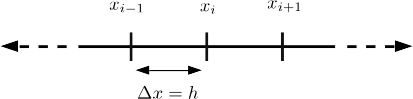
\includegraphics{lec17n-dx.png}
\caption{A discrete grid on which a function may be defined.}
\label{fig:lec17n-dx}
\end{marginfigure}
\section{First Derivative}
Consider a function defined on a discrete grid as shown in Figure \ref{fig:lec17n-dx}.  For simplicity of the following analysis, we will assume that the grid points are all equally spaced: $\Delta x = h$.  Suppose we know the value of the function,$f(x_i)$, at all grid points, $x_i$, and we wish to estimate the first derivative, $f^{\prime}(x_i)$.  From the Taylor series expansion we have:
\begin{multline*}
f(x_{i+1}) = f(x_i) + f^{\prime}(x_i)\overbrace{(x_{i+1}-x_i)}^{h} + \frac{f^{\prime \prime}(x_i)}{2!}\overbrace{(x_{i+1} - x_i)^2}^{h^2} + \cdots + \\ \frac{f^{(n)}(x_i)}{n!}\overbrace{(x_{i+1}-x_i)^n}^{h^n} + \cdots
\end{multline*}
If we solve for $f^{\prime}(x_i)$, we obtain a two-point \emph{forward difference} formula:
\begin{align*}
f^{\prime}(x_i) &= \frac{f(x_{i+1}) - f(x_i)}{h} - \text{higher order terms} \\
f^{\prime}(x_i) &= \frac{f(x_{i+1}) - f(x_i)}{h} - \frac{f^{\prime \prime}(\xi)}{2!}h
\end{align*}
in which it can be shown that the higher order terms are equal to $\frac{f^{\prime \prime}(\xi)}{2!}h$ with $\xi \in [x_{i},x_{i+1}]$.  We can more generically characterize that error term using asympototic notation: $\mathcal{O}(h)$.

We can similarly define a two-point backward difference formula:
\begin{align*}
f(x_{i-1}) &= f(x_i) - f^{\prime}(x_i)h + \frac{f^{\prime \prime}(x_i)}{2!}h^2 - \cdots \\
\Rightarrow f^{\prime}(x_{i}) &= \frac{f(x_i) - f(x_{i-1})}{h} + \mathcal{O}(h)
\end{align*}
These equations are simple to use and effective, however they have a significant drawback in that the error term is proportional to $h$.  For every extra decimal place we need to gain in accuracy, we must to reduce $h$ by a factor of 10.  This adds up quickly.  The good news is that we can do better.  

For first derivative formulas, we can try a centered difference scheme:\marginnote{


\vspace{2.3cm} 

\noindent Here we subtract the first equation from the second and solve for $f^{\prime}(x_i)$.
}
\begin{align*}
f(x_{i+1}) &= f(x_i) + f^{\prime}(x_i)h + \frac{f^{\prime \prime}(x_i)}{2!}h^2 + \mathcal{O}(h^3) \\
f(x_{i-1}) &= f(x_i) - f^{\prime}(x_i)h + \frac{f^{\prime \prime}(x_i)}{2!}h^2 - \mathcal{O}(h^3) \\
f^{\prime}(x_i) &= \frac{f(x_{i+1})- f(x_{i-1})}{2h} + \underbrace{\frac{\mathcal{O}(h^3)}{2h}}_{\mathcal{O}(h^2)}
\end{align*}
This results in second-order convergence.  We can also get second-order convergence if we use more data points in the derivation.  We will skip the messy algebraic details but three-point, second-order forward and backward differentiation formulas are given in Equation \ref{eq:lec17n-fdf}, and Equation \ref{eq:lec17n-bdf}.

\begin{equation}
f^{\prime}(x_{i}) = \frac{-3f(x_i) + 4f(x_{i+1}) - f(x_{i+2})}{2h}
\label{eq:lec17n-fdf}
\end{equation}

\begin{equation}
f^{\prime}(x_{i}) = \frac{f(x_{i-2}) - 4f(x_{i-1}) + 3f(x_i)}{2h}
\label{eq:lec17n-bdf}
\end{equation}

\vspace{0.5cm}

\noindent\textbf{Example: } Use the 2- and 3-point finite difference formulas to numerically differentiate $\cos{x}$.  

\vspace{0.1cm}

\noindent In this listing, we carry out the differentiation with 2-point difference methods. \marginnote[8.0cm]{

\noindent \ref{lst:ann17n-1} here we use these vectors to index \lstinline[style=myMatlab]{df_numeric} and \lstinline[style=myMatlab]{f} in a ``vectorized'' fashion rather than one equation at a time.
}
\begin{lstlisting}[style=myMatlab,name=lec17n-ex1]
clear
clc
close 'all'

f = @(x) cos(x);

n = 7;
Nx = 2^n;
xMin = 0; xMax = pi;
X = linspace(xMin,xMax,Nx);
h = X(2) - X(1);

% initialize the derivative array
df_numeric = nan(1,Nx); 

% use fwd difference at left end
df_numeric(1) = (1/h)*(f(X(2))- f(X(1)));

% use backward difference at right end
df_numeric(end) = (1/h)*(f(X(end)) - f(X(end-1)));

% use centered difference everywhere else
i = 2:(Nx-1); ip = i+1; im = i-1; /*!\annotation{lst:ann17n-1}!*/
df_numeric(2:(end-1)) = (1/(2*h))*(f(X(ip))-f(X(im)));

% plot the function and its derivative
Xp = linspace(xMin,xMax,10000);
figure(1)
plot(Xp,f(Xp),'-b',...
    X,df_numeric,'-r','linewidth',2);
grid on;
title('First Derivative of $\cos{x}$',...
    'fontsize',14,...
    'fontweight','bold','Interpreter','latex');
xlabel('X','fontsize',12,'fontweight','bold');
ylabel('Y','fontsize',12,'fontweight','bold');
legend('f(x)','f^{\prime}(x)');
set(gca,'fontsize',12,'fontweight','bold');
\end{lstlisting}
\begin{marginfigure}
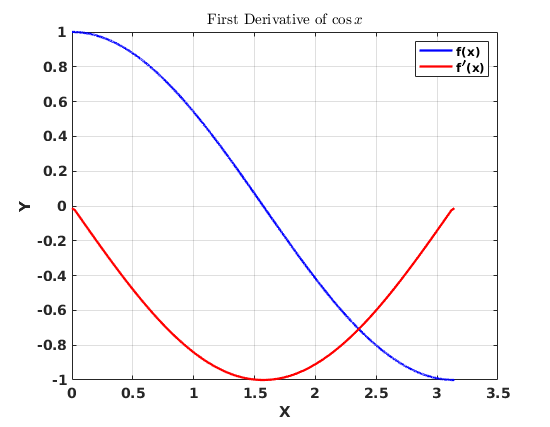
\includegraphics{lec17n-ex1-first-deriv.png}
\caption{A plot of $cos{x}$ and its first derivative calculated numerically.}
\label{fig:lec17n-ex1-first-deriv}
\end{marginfigure}

In the next listing a method for carrying out a convergence analysis is shown.
\begin{lstlisting}[style=myMatlab,name=lec17n-ex1]
%% Get Convergence Rate
N = 5:15;
rel_err = nan(1,length(N));
h_err = nan(1,length(N));

for s = 1:length(N)
    Nx = 2^N(s);
    xMin = 0; xMax = pi;
    X = linspace(xMin,xMax,Nx);
    h = X(2) - X(1);
    h_err(s) = h;
    
    df_numeric = nan(1,Nx);
    % use fwd difference at left end
    df_numeric(1) = (1/h)*(f(X(2))- f(X(1)));
    % use backward difference at right end
    df_numeric(end) = (1/h)*(f(X(end)) - f(X(end-1)));
    % use centered difference everywhere else
    i = 2:(Nx-1); ip = i+1; im = i-1;
    df_numeric(i) = (1/(2*h))*(f(X(ip))-f(X(im)));
    
    % estimate the relative error
    x_err = 1:Nx; % include the end points
    %x_err = 2:(Nx-1); % exclude the end points
   
    rel_err(s) = norm(df_numeric(x_err) - df(X(x_err)),2)...
        /norm(df(X(x_err)),2);    
end

% add gauge lines for convergence
c1 = 0;
h1 = h_err + c1;

c2 = 0;
h2 = h_err.^2 + c2;

figure(2)
loglog(h_err,rel_err,'-b',...
    h_err,h1,'--r',...
    h_err,h2,'--g','linewidth',3);
title('Convergence Behavior','fontsize',14,...
    'fontweight','bold');
xlabel('h','fontsize',12,'fontweight','bold');
ylabel('Relative Error','fontsize',12,'fontweight','bold');
grid on
set(gca,'fontsize',10,'fontweight','bold');
legend('Estimate','h^1 convergence','h^2 convergence',...
    'location','best');
\end{lstlisting}
We use the 2\textsuperscript{nd}-order accurate centered difference equation through most of the domain but, as Figure \ref{fig:lec17n-ex1-first-deriv-convergence} shows, the first-order accurate 2-point formulas at the end-points are enough to spoil convergence.

\begin{marginfigure}[-10.0cm]
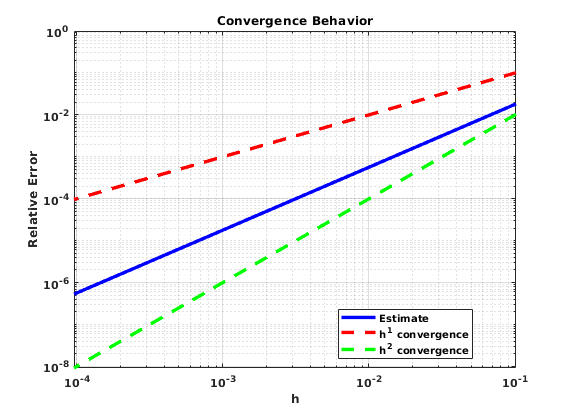
\includegraphics{lec17n-ex1-first-deriv-convergence.png}
\caption{Convergence behavior using 2-point finite difference formulas.}
\label{fig:lec17n-ex1-first-deriv-convergence}
\end{marginfigure}

If we use the 2\textsuperscript{nd}-order 3-point forward and backward differentiation formulas, we can get convergence at 2\textsuperscript{nd}-order as shown in Figure \ref{fig:lec17n-ex1-first-deriv-convergence2}.

\begin{marginfigure}[-3.0cm]
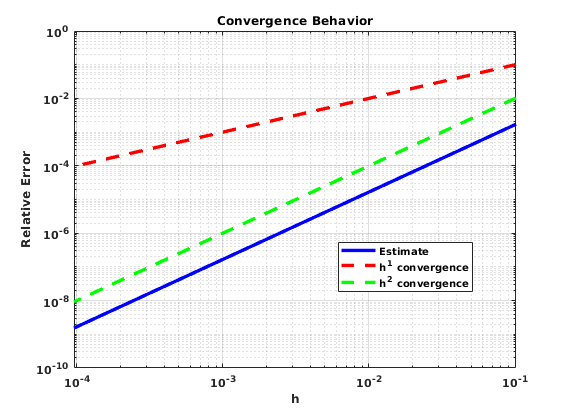
\includegraphics{lec17n-ex1-first-deriv-convergence2.png}
\caption{Convergence behavior using 2\textsuperscript{nd}-order finite difference equations throughout the domain.}
\label{fig:lec17n-ex1-first-deriv-convergence2}
\end{marginfigure}

\section{Second Derivative Formulas}

We can use finite difference equations to approximate the second derivative (and higher-order derivatives) as well.  As with first-order differentiation, we derive the formula from Taylor-series expansion.

\begin{align*}
f(x_{i+1})=f(x_i)+f^{\prime}(x_i)h+\frac{f^{\prime \prime}(x_i)h^2}{2!}+\frac{f^{\prime\prime\prime}(x_i)h^3}{3!}+ \cdots \\
f(x_{i-1})=f(x_i)-f^{\prime}(x_i)h+\frac{f^{\prime \prime}(x_i)h^2}{2!}-\frac{f^{\prime\prime\prime}(x_i)h^3}{3!}+ \cdots
\end{align*}
If we add the two equations above and solve for $f^{\prime \prime}(x_i)$, we get:
\begin{equation}
f^{\prime \prime}(x_i) = \frac{2f(x_{i-1})-2f(x_{i})+f(x_{i+1})}{h^2}+\mathcal{O}(h^2)
\end{equation}

